\documentclass[letterpaper,10pt]{article}

\usepackage{enumitem}
\usepackage{titling}
\usepackage{listings,listings-rust}
\usepackage{url}
\usepackage{soul}
\usepackage{hyperref}
\usepackage{setspace}
\usepackage{subfig}
\usepackage{sectsty}
\usepackage{pdfpages}
\usepackage{colortbl}
\usepackage{multirow}
\usepackage{multicol}
\usepackage{relsize}
\usepackage{amsmath}
\usepackage{wasysym}
\usepackage{fancyvrb}
\usepackage[yyyymmdd]{datetime}
\usepackage{amsmath,amssymb,amsthm,graphicx,xspace}
\usepackage[titlenotnumbered,noend,noline]{algorithm2e}
\usepackage[compact]{titlesec}
\usepackage{XCharter}
\usepackage[T1]{fontenc}
\usepackage[scaled]{beramono}
\usepackage[normalem]{ulem}
\usepackage{booktabs}
\usepackage{tikz}
\usetikzlibrary{arrows.meta,automata,shapes,trees,matrix,chains,scopes,positioning,calc,decorations.pathreplacing}
\tikzstyle{block} = [rectangle, draw, fill=blue!20, 
    text width=2.5em, text centered, rounded corners, minimum height=2em]
\tikzstyle{bw} = [rectangle, draw, fill=blue!20, 
    text width=4em, text centered, rounded corners, minimum height=2em]

\definecolor{namerow}{cmyk}{.40,.40,.40,.40}
\definecolor{namecol}{cmyk}{.40,.40,.40,.40}
\renewcommand{\dateseparator}{-}

\let\LaTeXtitle\title
\renewcommand{\title}[1]{\LaTeXtitle{\textsf{#1}}}

\lstset{basicstyle=\footnotesize\ttfamily,breaklines=true}

\newcommand{\CPP}{C\nolinebreak\hspace{-.05em}\raisebox{.4ex}{\tiny\bf +}\nolinebreak\hspace{-.10em}\raisebox{.4ex}{\tiny\bf +}}
\def\CPP{{C\nolinebreak[4]\hspace{-.05em}\raisebox{.4ex}{\tiny\bf ++}}}

\newcommand{\handout}[5]{
  \noindent
  \begin{center}
  \framebox{
    \vbox{
      \hbox to 5.78in { {\bf ECE459: Programming for Performance } \hfill #2 }
      \vspace{4mm}
      \hbox to 5.78in { {\Large \hfill #4  \hfill} }
      \vspace{2mm}
      \hbox to 5.78in { {\em #3 \hfill \today} }
    }
  }
  \end{center}
  \vspace*{4mm}
}

\newcommand{\lecture}[3]{\handout{#1}{#2}{#3}{Lecture#1}}
\newcommand{\tuple}[1]{\ensuremath{\left\langle #1 \right\rangle}\xspace}

\addtolength{\oddsidemargin}{-1.000in}
\addtolength{\evensidemargin}{-0.500in}
\addtolength{\textwidth}{2.0in}
\addtolength{\topmargin}{-1.000in}
\addtolength{\textheight}{1.75in}
\addtolength{\parskip}{\baselineskip}
\setlength{\parindent}{0in}
\renewcommand{\baselinestretch}{1.5}
\newcommand{\term}{Winter 2020}

\singlespace


\begin{document}

\lecture{23 --- Password Cracking, Reduced-Resource Computation}{\term}{Patrick Lam \& Jeff Zarnett}

\section*{GPU Application: Password Cracking}

GPUs are good---too good, even---at password cracking. We'll discuss a paper
that proposes a technique to make it harder to crack passwords. This technique
is scrypt, the algorithm behind DogeCoin~\cite{scrypt}. See also \url{http://www.tarsnap.com/scrypt.html}

First, let's talk about acceptable practices for password storage. It is \emph{not}
acceptable engineering practice to store passwords in plaintext. The inevitable security
breach will end with your company sending a ``sorry'' disclosure email to its clients,
and you will be responsible for the ensuing bad publicity.

Acceptable practices: {\bf not} plaintext; hashed and salted (we won't discuss salting here but hopefully you remember it from previous courses or other experience.)

\paragraph{Cryptographic hashing.} Instead of storing the plaintext password, you
store a hash of the password, under a cryptographic hash function. One important
property of a cryptographic hash function is that it must be (believed to be a) one-way
function; that is: $x \mapsto f(x)$, the forward direction, must be easy to compute, but
$f(x) \mapsto x$, the inverse mapping, must be hard to compute. Examples of such functions
include SHA1 and scrypt.

\paragraph{Not Secret.}
In real life, you can get around the idea of cryptographic hashing by looking on the internet to see if someone's password has already been leaked. Many services are terrible about their password storage policies so if you used the same username and password combination of mycrappywebsite.com and your online banking, then if the mycrappywebsite database gets hacked then the attacker has your user and password already without having to break anything.

\paragraph{First, Check if the Door Is Locked}
As you might imagine, the first thing to try is super common passwords: ``password'', ``system'', et cetera. Users frequently choose common words as passwords and if you just try them all you might get a hit. Choose stronger passwords!

\paragraph{Breaking the hash.} Even if there is no known short computation for the
inverse function, it's always possible to brute-force the password
computation by trying all possible passwords. Think about how GPUs
work. Each potential password is a point in the computation space, and
we compute the hash over all of them simultaneously.  That's a lot of
speedup. Custom hardware is also good, and those of you who know
something about hardware could think about implementing
it. Oh, hello, Bitcoin miners (but don't actually mine Bitcoin, please).

\paragraph{Arms race: making cracking difficult.} The idea has always been
to make it more difficult to compute the hash function, so that it's OK to
try one password, but it's intractable to try one billion passwords. Even way back,
UNIX passwords forced repeated applications of the hash function to accomplish these.

The main idea behind scrypt is to make hashing expensive in both time and space,
increasing both the number of operations and the cost of brute-forcing.
Hence crackers will need to use more circuitry to break passwords.

Of course, there's always this form of cracking:
\begin{center}
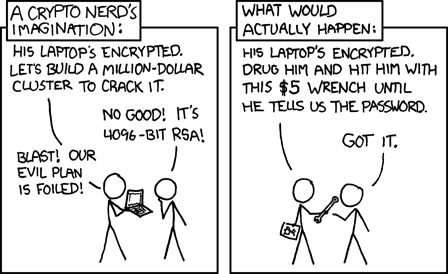
\includegraphics[width=0.5\textwidth]{images/xkcd-538}\\
\hfill (Source: xkcd 538)
\end{center}

\newtheorem{defn}{Definition}

\paragraph{Formalization.} Let's make the notion of ``expensive'' a bit more formal.
The idea is to force the use of the ``most memory possible'' for a given number of
operations. More memory implies more circuitry required to implement.

    \begin{defn}
      A \emph{memory-hard} algorithm on a Random Access Machine is an
      algorithm which uses $S(n)$ space and $T(n)$ operations, where
      $S(n) \in \Omega(T(n)^{1-\varepsilon})$.
    \end{defn}

Memory-hard algorithms are expensive to implement in either hardware or software.

Now, we want to move from particular algorithms to the underlying
functions (that is, we would like to quantify over all possible
algorithms). Intuitively, a \emph{sequential memory-hard function} is
one where (1) the fastest sequential algorithm is memory-hard; and (2)
it is impossible for a parallel algorithm to asymptotically achieve
lower cost.

\paragraph{Existence proof.} Of course anyone can define anything.
It's much better if the thing being defined actually exists. The
scrypt paper then goes on to exhibit ReMix, which is a concrete
example of a sequential memory hard function.

Finally, the paper concludes with an example of a more realistic
(cache-aware) model and a hard function in that context, BlockMix.

\paragraph{Rainbow Tables} So, the brute force approach is the simplest to describe but is computationally intensive, and if a sufficiently-well-designed cryptographic hash function is used it's really tough to actually crack a password. But maybe if we want to crack a password we don't have to always start from zero; maybe we could remember some previous computations so that we could use those answers later. If we calculated the hash of password ``12345'' and we knew what that looked like, if we encountered that hash in the future we could already jump immediately to the answer in our lookup table. This is the basic idea behind \textit{rainbow tables}.

There is a technical paper describing how rainbow tables work, but we'll instead use a much less cryptograhic-expert-level explanation~\cite{rainbowtables}. 

Part of the difficulty with this approach is that it isn't practical, or even really possible, to store the hashes for every possible plaintext (unless the plaintext is very small). So the rainbow table is a compromise between speed and space. The ``reduction'' function maps hashes to plaintext:

\begin{center}
	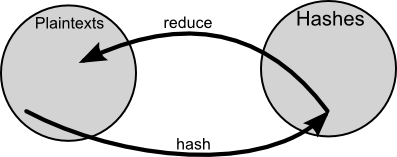
\includegraphics[width=0.4\textwidth]{images/rainbow-tables-reduce.png}\\
	Showing the reduce and hash functions~\cite{rainbowtables}.
\end{center}

This mapping function isn't the inverse of the hash function; it's just some sort of categorization. If the set of passwords to be cracked is, say, six digit numeric, then we compute the hash for a given input (``123456'') and we get some output (``d41d8cd98f00b204e9800998ecf8427e'') which is then reduced (mapped) to some other value (e.g., we'll take the first 6 numbers, 418980). We have another plaintext now, 418980. So we hash this new one, and reduce it, and so on and so on, until some end point ($n$ times, where you choose $n$). 

\begin{center}
	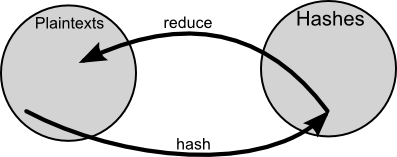
\includegraphics[width=0.4\textwidth]{images/rainbow-tables-reduce.png}\\
	And now we have a chain~\cite{rainbowtables}.
\end{center}

We should do this to develop some number of chains. This is the sort of task you could do with a GPU, because they can do a reduction relatively efficiently. 

Once we have those developed for a specific input set and hash function, they can be re-used forever. You do not even need to make them yourself anymore (if you don't want) because you can download them on the internet... they are not hard to find. They are large, yes, but in the 25 - 900 GB range, which is large  but not ridiculous. I mean, Fallout 76 had a day one patch of 52 GB, and it was a disaster of a game.

Alright, so, you've got them (or made them), but how do we use rainbow tables? Well, for a given hash with an unknown plaintext~\cite{rainbowtables}:
\begin{enumerate}
	\item Look for the hash in the list of final hashes; if there, we are done
	\item If it's not there, reduce the hash into another plaintext and hash the new plaintext
	\item Go back to step 1
	\item If the hash matches a final hash, the chain with the match contains the original hash
	\item Having identified the correct chain, we can start at the beginning of the chain with the starting plaintext and hash, check to see if we are successful (if so, we are done); if not, reduce and try the next plaintext. 
\end{enumerate} 

Like generation, checking the tables for a hit can also be done efficiently by the GPU. Some numbers from \url{http://www.cryptohaze.com/gpurainbowcracker.php.html}: 
\begin{itemize}
	\item Table generation on a GTX295 core for MD5 proceeds at around 430M links/sec.
	\item Cracking a password 'K\#n\&r4Z': real: 1m51.962s, user: 1m4.740s. sys: 0m15.320s
\end{itemize}

Yikes. There is obviously a little bit more complexity to how the rainbow tables work (such as dealing with collisions and loops), but it is clear just how devastatingly effective GPU computations are on breaking passwords.

\section*{The N-Body Problem and Reduced-Resource Computation}
A common physics problem that programmers are asked to simulate is the N-Body problem: you have some number of bodies (N!) and they interact via gravitational forces. The program needs to compute the movements of the bodies over time. This is a typical example of a program that is well suited to OpenCL: you can compute the forces on each body $n$ from all other bodies in parallel. This was even at one time an assignment in this course, although now there are too many good solutions on the internet so it was replaced. Ah well.

Once you've made the conversion to OpenCL and let's assume you've optimized it well so far. What can you do here if you want to speed it up even more? You could look for optimizations that trade off accuracy for performance. As you might imagine, using \texttt{float} instead of \texttt{double} can save half the space which should make things quite a bit faster. But you want more...

In the specific case of the N-body simulation,
domain knowledge would enable you to skimp out on
some unnecessary computation: points that are far away contribute only
very small forces. So you can estimate them (crudely). The idea is to divide the points into a number of ``bins'' which are cubes representing a locale of some sort. Then, compute the centre of mass for each bin. When calculating the forces on a given point, add the force exerted by the centre of mass for faraway bins to the force exerted by individual particles for nearby particles.

A more concrete explanation with an example: suppose the space  is divided into $[0, 1000]^3$, so we can take bins which are cubes of length 100. This gives 1000 bins. If you want to increase the accuracy, increase the number of bins. If you want to increase the speed, decrease the number of bins.

The program should have a 3-dimensional array {\tt cm} of {\tt
  float4}s to store centres-of-mass. The {\tt x}, {\tt y} and {\tt z}
components contain the average position of the centres of mass of a
bin, while the {\tt w} component stores the total mass. Compute all of
the masses in parallel: create one thread per bin, and add a point's
position if it belongs to the bin, e.g.

\begin{lstlisting}
    int xbin, ybin, zbin; // initialize with bin coordinates
    int b;
    for (i = 0; i < POINTS; i++) {
        if (pts[i] in bin coordinates) {
            cm[b].x += pts[i].x; // y, z too
            cm[b].w += 1.0f;
        }
    }
    cm[b].x /= cm[b].w; // etc
\end{lstlisting}

 \noindent
Note that this parallelizes with the number of bins.

For the next step, the program needs to keep track of the points in
each bin. Fortunately, you've collected the number of points in each
bin, so you can allocate the appropriate amount of memory to store the
points in a two-dimensional array {\tt binPts}. In a second phase,
iterate over all bins again, this time putting coordinates into the
proper element of {\tt binPts}.


The payoff from all these calculations is to save time while
calculating forces. In this example, we'll compute exact
forces for the points in the same bin and the directly-adjacent bins
in each direction (think of a Rubik's Cube; that makes 27 bins in all,
with 6 bins sharing a square, 12 bins sharing an edge, and 8 bins
sharing a point with the centre bin). If there is no adjacent bin 
(i.e., this is an edge), just act as if there are no points 
in the place where the nonexistent bin would be. 

Necessarily, writing the program like this is going to mean more than one kernel.
Each discrete step (compute centre of mass, put coordinates into bins, 
calculate forces) will be different kernels. This does mean there is overhead for each kernel, meaning the total amount of overhead goes up. Is it worth it? Let's see the data from a reference solution [PL] for the previous assignment:

\paragraph{With 500*64 points.}
\begin{itemize}
\item    OpenCL, no approximations (1 kernel): 0.182s
\item    OpenCL, with approximations (3 kernels): 0.168s
\end{itemize}
 \paragraph{With 5000*64 points.}
\begin{itemize}
\item    OpenCL, no approximations (1 kernel): 6.131s
\item    OpenCL, with approximations (3 kernels): 3.506s
\end{itemize}

\subsection*{Early phase termination}

In~\cite{Rinard:2010:PSA:1932682.1869525}, Martin Rinard summarizes
two of his novel ideas for automatic or semiautomatic optimizations
which trade accuracy for performance: early phase
termination~\cite{Rinard:2007:EarlyPhaseTermination} and loop
perforation~\cite{hoffmann09:_using_code_perfor_improv_perfor}. Both
of these ideas are applicable to code we've learned about in this
class.


We've talked about barriers quite a bit. Recall that the idea is that
no thread may proceed past a barrier until all of the threads
reach the barrier. Waiting for other threads causes delays. 
Killing slow threads obviously speeds up the program. Well, that's easy.

\begin{center}
``Oh no, that's going to change the meaning of the program!''
\end{center}

Let's consider some arguments about when it may be acceptable to just
kill (discard) tasks. Since we're not completely crazy, we can develop
a statistical model of the program behaviour, and make sure that the
tasks we kill don't introduce unacceptable distortions. Then when we
run the program, we get an output and a confidence interval.

\paragraph{Two Examples.} When might this work? Monte Carlo simulations
are a good candidate; you're already picking points randomly.
Raytracers can work as well. Both of these examples could spawn a lot
of threads and wait for all threads to complete.  In either case, you
can compensate for missing data points, assuming that they look like
the ones that you did compute. If you have a function where some graph is being
computed, you can probably guess that a missing point is somewhere in between
the two adjacent points.

The same is true for graphics, of course: if rendering a particular pixel did
not go well for some reason, you can just average the adjacent ones and probably
people would not notice the difference. Not bad!

Also recall that, in scientific computations, you're entering points
that were measured (with some error) and that you're computing
using machine numbers (also with some error). Computers are only
providing simulations, not the ground truth; the question is
whether the simulation is good enough.

\subsection*{Loop perforation} 
You can also apply the same idea to sequential programs. Instead
of discarding tasks, the idea here is to discard loop iterations.
Here's a simple example: instead of the loop,
\begin{center}
\verb|for (i = 0; i < n; i++) sum += numbers[i];|
\end{center} \vspace*{-1em}
simply write,
\vspace*{-1em}\begin{center}
\verb|for (i = 0; i < n; i += 2) sum += numbers[i];|
\end{center}
and multiply the end result by a factor of 2. This only works 
if the inputs are appropriately distributed, but it does give a
factor 2 speedup.

\paragraph{Example domains.} In~\cite{Rinard:2010:PSA:1932682.1869525},
we can read that loop perforation works for evaluating forces on water
molecules (in particular, summing numbers); Monte-Carlo simulation for
swaption pricing; and video encoding. In that example, changing loop
increments from 4 to 8 gives a speedup of 1.67, a signal to noise ratio
decrease of $0.87\%$, and a bitrate increase of $18.47\%$, producing
visually indistinguishable results. The computation looks like this:

{\small
\begin{verbatim}
min = DBL_MAX;
index = 0;
for (i = 0; i < m; i++) {
  sum = 0;
  for (j = 0; j < n; j++) sum += numbers[i][j];
  if (min < sum) {
    min = sum;
    index = i;
  }
}
\end{verbatim}
}
The optimization changes the loop increments and then compensates. 


\bibliographystyle{alphaurl}
\bibliography{459}


\end{document}
